\section{NLIZE System}
In this section, we discuss the design and implementation of the NLIZE (pronounced as ``analyze''; see interface overview in Fig.~\ref{fig:teaser}) system, which address the visualization tasks (\textbf{T1-3}).
%
As discussed in the task analysis, the experts often analyze and obtain intuition about the model by studying how altering one part of the model affects other stages of the pipeline.
%
Such a process can be generalized as the perturbation-driven paradigm, which is used as a guiding principal for designing the proposed tool.
%
As illustrated in Fig.~\ref{fig:modelPipeline}, we enable the automated or user-guided \emph{perturbation} (i.e., replace words) of the input sentence, the \emph{perturbation} of attention (i.e., alter the alignment between sentences) inside the model, and the \emph{perturbation} of the prediction (e.g., adjust the prediction by making updates to the model).
%
In the following sections, we describe in detail the five major components of the proposed system, namely, the sentence view  (Section~\ref{sec:sentence}), the attention view (Section~\ref{sec:attention}), the prediction view (Section~\ref{sec:prediction}), the pipeline view (Section~\ref{sec:pipeline}), and the all pair summary view (Section~\ref{sec:allPairs}).


\begin{figure}[htbp]
\centering
 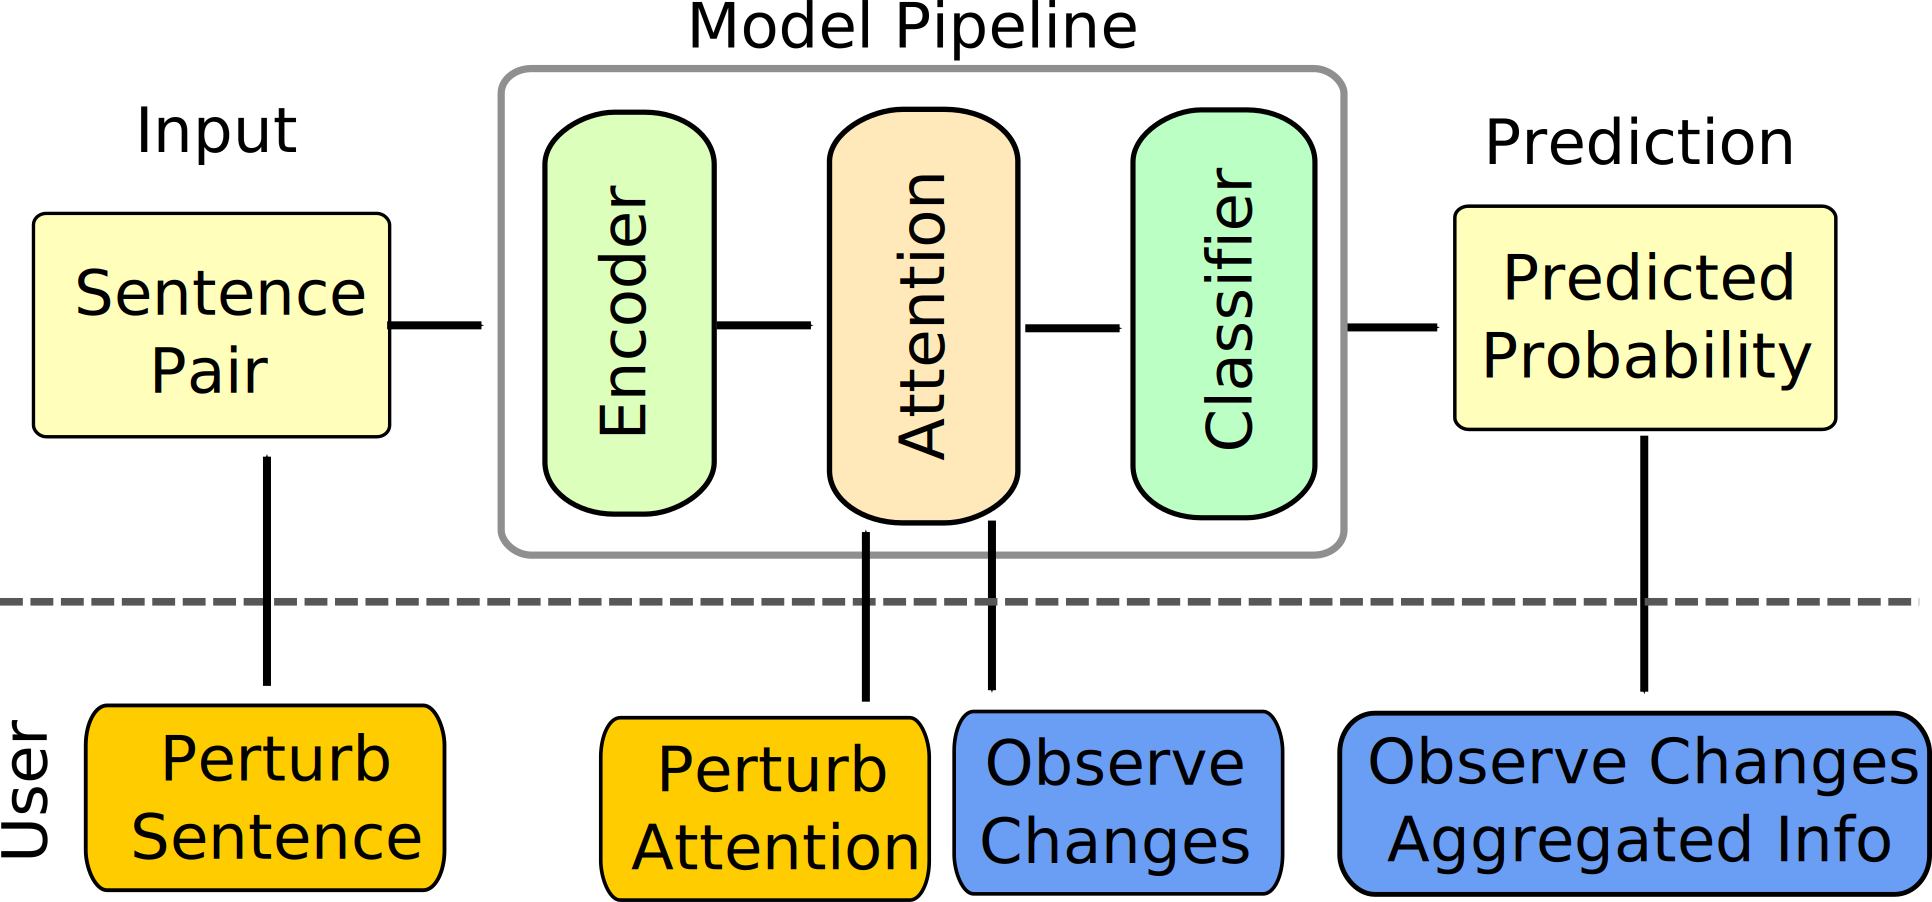
\includegraphics[width=1.0\linewidth]{pipeline}
 \caption{
 Perturbation-driven exploration of the natural language inference model.
 In the proposed tool, we enable the interrogation of the relationship between different components of the model via the perturbation-based analysis.
 %
 The user can perturb the input sentences (i.e., replace words with synonymous), perturb the attention (i.e., alter the soft alignment between sentences), and perturb the prediction (i.e., adjust the prediction by making updates to the model).
}
\label{fig:modelPipeline}
\end{figure}

% Beside looking into the internal states, understanding how each of the component of the model interact with input and output as well as with each other is the crucial for truly examine the mechanism of the model.
%
% Look at how the model work in action and interrogate relationship between different component, i.e., how the change made to one part of model affect the other pieces present, is the key to gain the full picture.

%%% Local Variables:
%%% mode: latex
%%% TeX-master: "paper_entailVis"
%%% End:
